\documentclass[12pt]{article}
\usepackage[utf8]{inputenc}
\usepackage{amsmath}
\usepackage{graphicx}
\usepackage{hyperref}
\usepackage[spanish]{babel}
\usepackage{parskip}  % Paquete para controlar la sangría y el espaciado entre párrafos
\usepackage{graphicx}  % Paquete para incluir imágenes
\usepackage{tocbibind}  % Para incluir el índice de imágenes en el índice general
\usepackage{amsfonts}
\usepackage{float}

\setlength{\parindent}{1em}  % Establece la sangría de los párrafos
\setlength{\parskip}{0.5em}   % Establece el espaciado entre los párrafos

\title{\Huge Visión Artificial}
\author{\Large Juan Diego Gallego Nicolás\\ \href{mailto:jdiego.gallego@um.es}{jdiego.gallego@um.es}}
\date{\Large 23/03/2025}

\begin{document}

\maketitle
\thispagestyle{empty}

% Portada
\begin{center}
    \vspace{2cm}
    \textbf{Entrega Parcial}
\end{center}

\newpage

% Índice
\tableofcontents
\newpage

% Índice de imágenes
\listoffigures
\newpage

% Sección 1: Introducción
\section{Introducción}
Este documento recoge explicaciones y resultados de los ejercicios realizados durante el desarrollo de la asignatura
siguiendo las instrucciones del repositorio de GitHub albertoruiz/umucv/blob/master/notebooks/ejercicios.ipynb (revisado el 20/03/2025).
Cada ejercicio se corresponde con la sección del documento con el mismo nombre.
A su vez, cada sección se divide en los subapartados: Marco Teórico, Resultados y Comentarios.

La sección Marco Teórico servirá como resumen de los contenidos teóricos desarrollados en la teoría necesarios para la realización de la práctica. 
A continuación, en el apartado de Resultados se hablará del trabajo realizado (código y pruebas) y de cómo se han aplicado los conocimientos teóricos.
Finalmente, la sección Comentarios se reserva para realizar alguna reflexión y plasmar las conclusiones y opiniones sobre el ejercio.

Las imágenes incluidas son extraídas de:
\begin{itemize}
    \item Geogebra clásico: www.geogebra.org/classic?lang=es
    \item Geogebra 3D: www.geogebra.org/3d?lang=es
    \item Material de la asignatura: material de la asignatura
    \item Gráficas generadas con matplotlib
    \item Cámara de un Google Pixel 8 Pro
    \item Google Earth
\end{itemize}

A lo largo del documento se hará mención a una serie de scripts de python desarrollados por el profesor Alberto Ruiz. Estos scripts se encuentran en el repositorio de GitHub albertoruiz/umucv/ (revisado el 20/03/2025).

\newpage

% Sección 2: Calibración
\section{Calibración}

\subsection{Calibración: Marco Teórico}

Una cámara es un dispositivo compuesto esencialmente por una lente que enfoca luz en un plano de proyección.
Ese plano de proyección físico se sitúa detrás de la lente y tomando la imagen de forma invertida. Tras deshacer la inversión, los dispositivos de visualización presentan la imagen en la orientación correcta.
Nótese que el proceso de reconstrucción de la imagen genera un plano de proyección virtual con las mismas dimensiones y a la misma distancia a la lente que el plano real \ref{fig:Modelo_camara}.

\begin{figure}[h!]
    \centering
    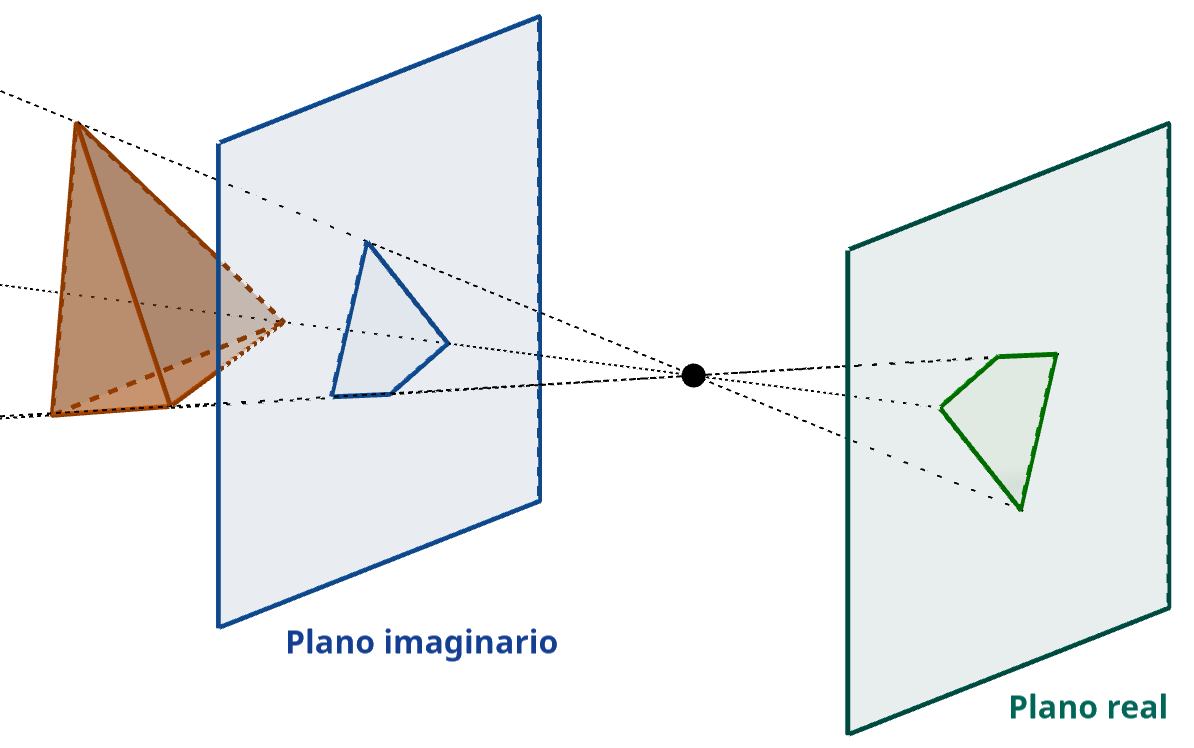
\includegraphics[width=0.7\textwidth]{images_calibracion/Modelo_camara.png}  % Cambia 'imagen_ejemplo.jpg' por el nombre de tu archivo
    \caption{Modelo de una cámara.}
    \label{fig:Modelo_camara}
\end{figure}

Hay dos parámetros esenciales que describen las propiedades de una cámara: su resolución y su distancia focal. 
La resolución hace referencia a las dimensiones del plano de proyección.
Esta se mide en píxeles (unidad mínima de representación de color) y se puede presentar como el par $W \times H$ o como el número de total píxeles en el plano.
La distancia focal es la distancia entre el foco de la lente y el plano de proyección. También se mide en píxeles.

Calibrar la cámara consiste en aproximar lo máximo posible estos parámetros. Una vez conocidos, se pueden hacer mediciones en el mundo real de distancias, dimensiones y ángulos como veremos más adelante. 
En el caso de esta práctica, usaremos un patrón cuadriculado para este proceso \ref{fig:cuadricula}, aprovechando las distorsiones de tamaños y de los ángulos rectos.

\begin{figure}[h!]
    \centering
    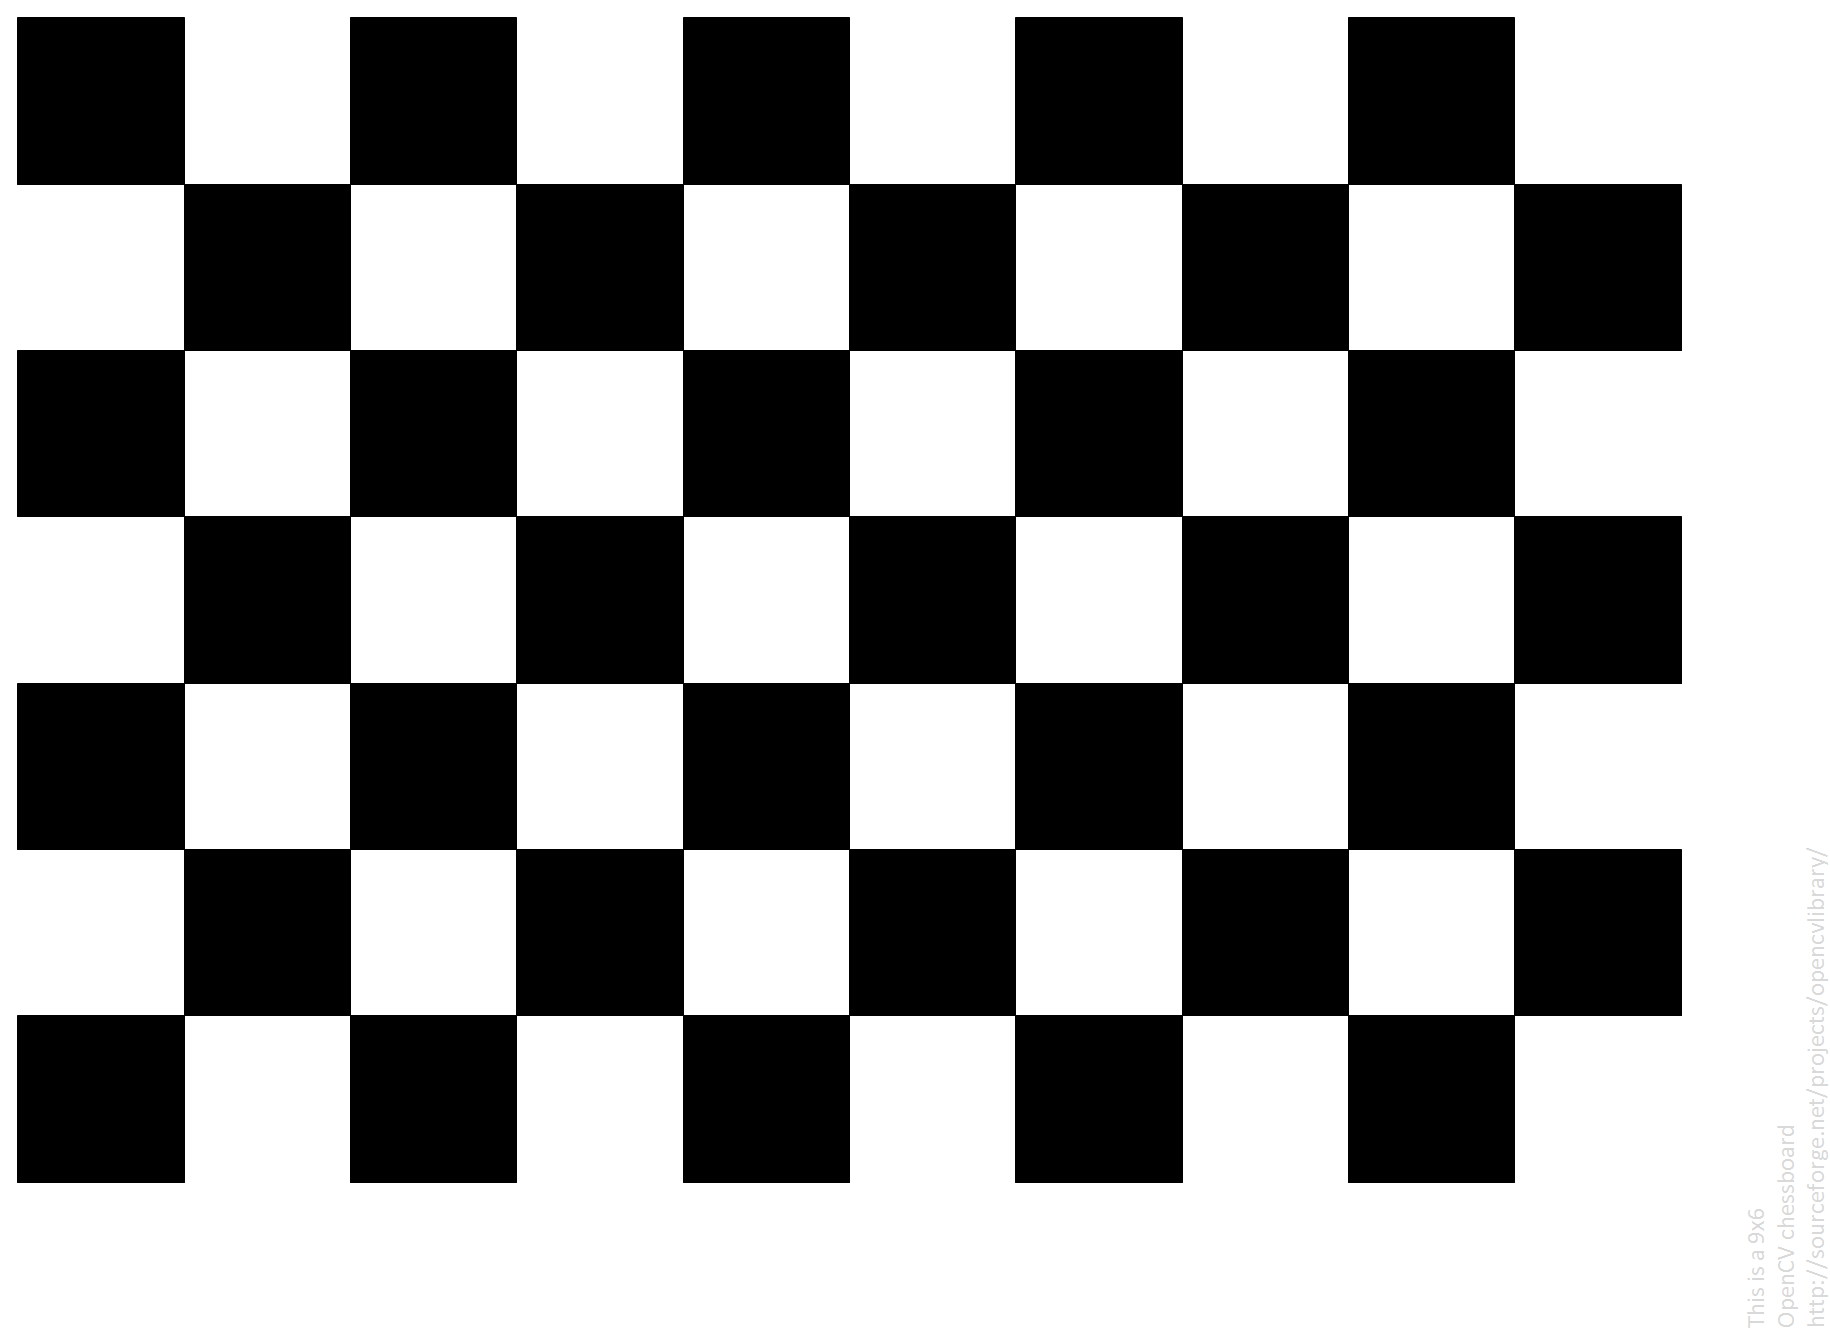
\includegraphics[width=0.7\textwidth]{images_calibracion/Patron_calibracion.png}  % Cambia 'imagen_ejemplo.jpg' por el nombre de tu archivo
    \caption{Patrón para la calibración de la cámara.}
    \label{fig:cuadricula}
\end{figure}

El proceso de calibración da como resultado una matriz $K \in \mathcal{M}_{3 \times 3} (\mathbb{R})$:
$$
K=
\begin{bmatrix}
f & 0 & o_x \\
0 & f_r & o_y \\
0 & 0 & 1
\end{bmatrix}
$$
donde:
\begin{itemize}
    \item[--] $f, f_r$ es la distancia focal y un valor cercano
    \item[--] $(o_x,o_y)$ son las coordenadas en las que se sitúa la proyección del foco de la cámara (normalmente $(W/2,H/2)$)
\end{itemize}

Una propiedad de la cámara interesante, derivada de los parámetros anteriores, es el campo de visión o FOV (Field Of View). 
Es una medida angular que representa las amplitudes horizontal y veltical máximas reconocibles por la cámara \ref{fig:Modelo_fov}.
Aplicando trigonometría básica se derivan las siguientes fórmulas para el FOV horizontal y vertical:
$$ FOV_H = 2*arctan \left( \frac{w}{2f} \right) \text{;     } FOV_V = 2*arctan \left( \frac{h}{2f} \right)$$ 
\begin{figure}[h!]
    \centering
    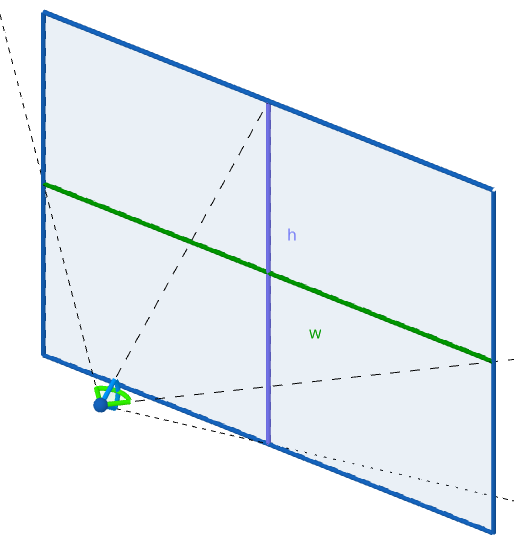
\includegraphics[width=0.7\textwidth]{images_calibracion/Modelo_fov.png}  % Cambia 'imagen_ejemplo.jpg' por el nombre de tu archivo
    \caption{FOV}
    \label{fig:Modelo_fov}
\end{figure}
También, a partir del FOV se deduce la unidad angular mínima medible como $\frac{FOV_H}{W} = \frac{FOV_V}{H}$.

La última propiedad que necesitamos para la realización de la práctica es la relación entre tamaño, tamaño aparente, distancia a la lente y distancia focal.
Esta la podemos obtener aplicando el Teorema de Tales aplicado a los triángulos formados por el foco de la cámara y los pares de extremos reales y virtuales del objeto proyectado \ref{fig:Tales}. 

Claro está que para que esto funcione el objeto a medir ha de estar lo más centrado posible, ya que en los extremos de la imagen se produce distorsión. En las imágenes tomadas para este proyecto se han intentado centrar lo máximo posible los objetos de interés evitando así dicho efecto.

\begin{figure}[H]
    \centering
    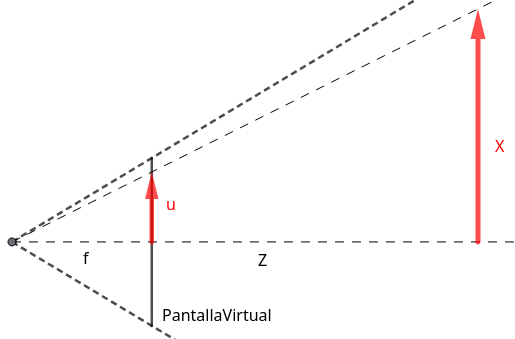
\includegraphics[width=0.6\textwidth]{images_calibracion/Tales.png}  
    \caption{Medidas sobre la imagen.}
    \label{fig:Tales}
\end{figure}

\subsection{Calibración: Resultados}

La realización de los ejercicios se puede ver en el notebook de python 'calibracion.ipynb'. 

\subsubsection{Obtención de la matriz de calibración}

El primer paso para la realización de la práctica es la calibración de la cámara. 
Para comenzar, he utilizado el programa 'stream.py' para tomar imágenes del patrón \ref{fig:cuadricula} desde una variedad de posiciones y ángulos \ref{fig:calibracion}. 
\begin{figure}[H]
    \centering
    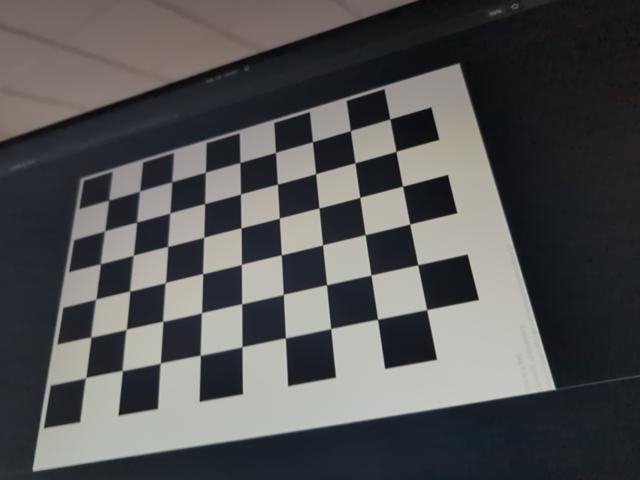
\includegraphics[width=0.4\textwidth]{images_calibracion/Calibracion.png}
    \caption{Fotografía tomada para calibración.}
    \label{fig:calibracion}
\end{figure}
Es importante que exista una variedad en los ángulos de captura ya que la funcionalidad findChessboardCorners de OpenCV utiliza la distorsión en los ángulos de las esquinas de los cuadrados para calcular los parámetros que buscamos.

Una vez tenemos las imágenes, usamos el programa 'calibracion.py' para calibrar la cámara, dando como resultado la matriz de calibración:
$$
K=
\begin{bmatrix}
    561.11 & 0.0000 & 317.80 \\
    0.0000 & 561.09 & 234.53 \\
    0.0000 & 0.0000 & 1.0000
\end{bmatrix}
$$
para una resolución de $640 \times 480$. Con los programas 'triangulate.py' y 'verify.py' podemos comprobar que el proceso se ha completado con éxito.

\subsubsection{FOV y pista de baloncesto}

Con la distancia focal obtenida podemos calcular el $FOV$ de la cámara:
$$FOV_H = 2*arctan \left( \frac{w}{2f} \right) = 59.39^{\circ}$$ 
$$FOV_V = 2*arctan \left( \frac{h}{2f} \right) = 46.32^{\circ}$$
Con este valor, podemos calcular la altura a la que tendríamos que situar la cámara para capturar por completo una pista de baloncesto a partir de sus dimensiones ($28 \times 15$ metros):
$$
tan \left( \frac{FOV_H}{2} \right) = \frac{28/2}{h_1} \Rightarrow h_1 = \frac{14}{tan(FOV_H/2)}=24.5485625m
$$
$$
tan \left( \frac{FOV_V}{2} \right) = \frac{15/2}{h_2} \Rightarrow h_2 = \frac{7.5}{tan(FOV_V/2)}=17.5346875m
$$
De entre los dos resultados tenemos que tomar el mayor, pues necesitamos que la pista se vea tanto a lo largo como a lo ancho.

Buscando el tamaño del resto de líneas de la pista podemos hacer una representación en 3D que nos hace a la idea de la situación que experimentaría la cámara en estas condiciones \ref{fig:pista_basket}:
\begin{figure}[H]
    \centering
    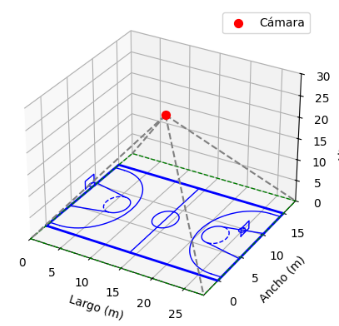
\includegraphics[width=0.4\textwidth]{images_calibracion/Pista_basket.png}
    \caption{Cámara sobre la pista de baloncesto.}
    \label{fig:pista_basket}
\end{figure}
Como se puede observar, sobra espacio mas a allá bandas debido a que la altura necesaria para ver la distancia entre los laterales era menor. 
También se intuye que al estar a una determinada altura las canastas no son entran dentro de la pirámide que constituye el espacio de visión de la cámara.
Aun así, posteriormente supondremos que las canastas se encuentran a nivel de suelo.

\begin{figure}[H]
    \centering
    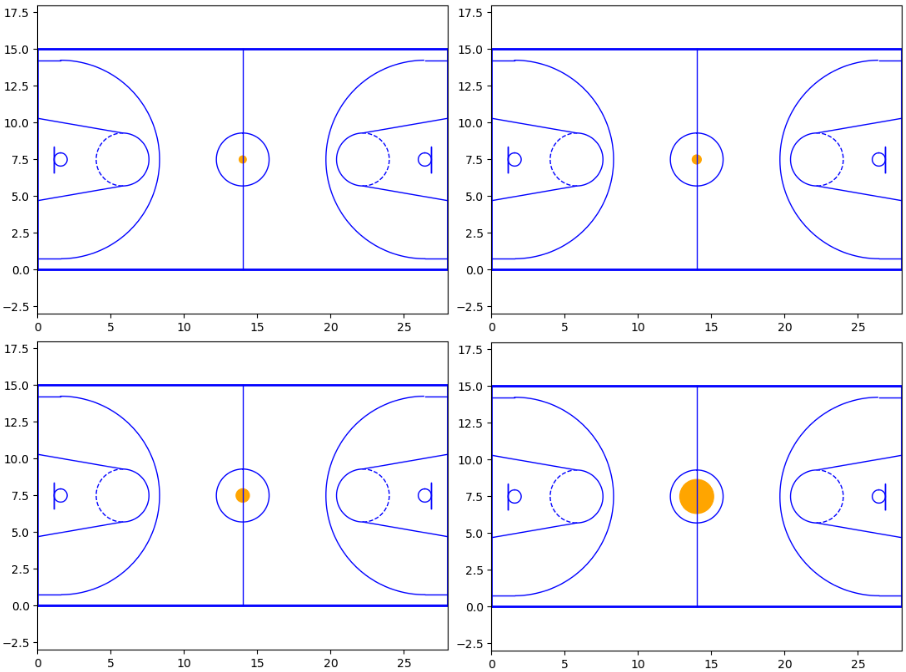
\includegraphics[width=0.75\textwidth]{images_calibracion/Pelota.png}  
    \caption{Pelota al 0\%, 25\%, 50\% y 80\% de la altura de la cámara.}
    \label{fig:pelota}
\end{figure}

En la imagen anterior \ref{fig:pelota} aprovechamos el modelo de la pista para simular el tamaño de una pelota de baloncesto situada a diferentes alturas del círculo central.
Para la primera instancia, el tamaño de la pelota ($48 cm$ de diámetro) es muy pequeño en comparación de la pista. En el tramo de 0\% a 50\% el tamaño aparente solo se duplica ya que esta magnitud es inversamente proporcional a la distancia a la cámara.
Al 80\% de la distancia al suelo el tamaño se ha multiplicado por $5$. Para valores más altos la pelota empieza a ser demasiado grande como para caber en el espacio visual de la cámara.

\subsubsection{Medir objetos}

Vamos ahora a explorar ahora las posibilidades de la relación
$$
\frac{u}{f} = \frac{X}{Z}
$$
utilizando la herramienta 'mouse.py' desarrollada en las prácticas que nos permite medir distancias en una imagen conociendo la matriz de calibración.

En primer lugar, podemos predecir la altura en píxeles que tendrá una persona a una cierta distancia de la cámara. 
Por ejemplo, en la imagen \ref{fig:altura_persona} aparezco yo mismo situado a $7.2$ metros de la cámara. Sabiendo que mi altura es de $1.74$ metros mi tamaño aparente debería de ser:
$$u=\frac{X}{Z} \times f = \frac{1.74}{7.2} \times 561.11 = 135.60 px$$
Por tanto, la altura medida entra dentro de la precisión esperada.

\begin{figure}[H]
    \centering
    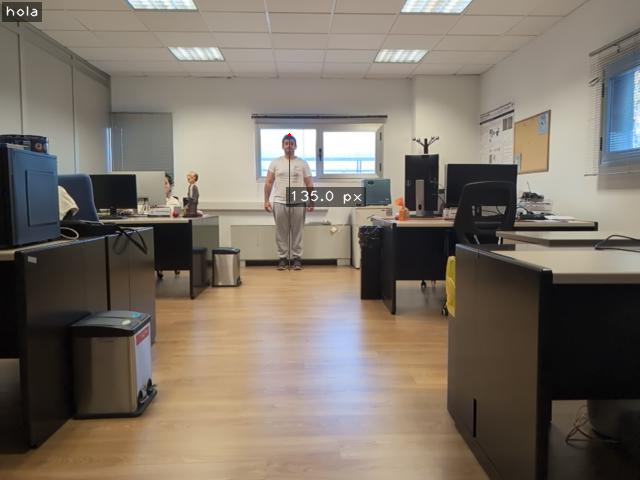
\includegraphics[width=0.6\textwidth]{images_calibracion/Altura_persona.png}  
    \caption{Altura de una persona}
    \label{fig:altura_persona}
\end{figure}

Por otro lado, vamos a intentar medir un objeto directamente con la cámara.
Para ello, situamos un muñeco a $19.5cm$ de la cámara y utlizamos el mismo programa para medir su tamaño aparente \ref{fig:altura_objeto}.
\begin{figure}[H]
    \centering
    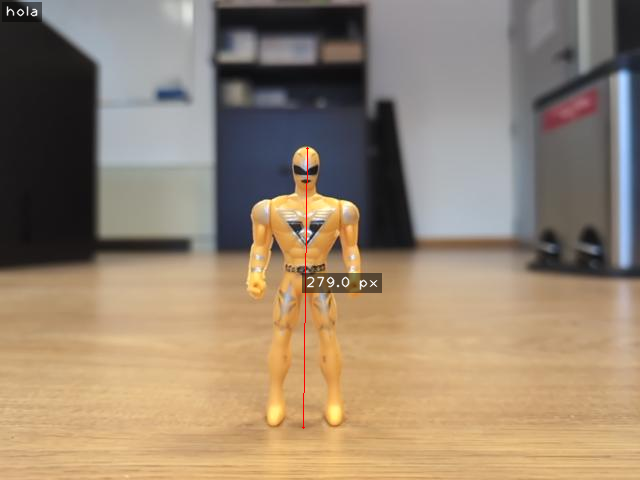
\includegraphics[width=0.6\textwidth]{images_calibracion/Altura_objeto.png}  
    \caption{Tamaño de un objeto}
    \label{fig:altura_objeto}
\end{figure}
Con el dato de $279px$ utilizamos la misma relación para obtener el tamaño del muñeco:
$$X = \frac{u}{f} \times Z= \frac{279}{561.11} \times 19.5 = 9.7 cm$$
lo que coincide con el tamaño real con una precisión milimétrica.

Lo último que podemos hacer directamente con esta relación es calcular la distancia a la que se encuentra un objeto cuyas dimensiones conocemos. Por ejemplo, un coche que mida 4 metros de largo y que ocupe 20 píxeles en pantalla estará a una distancia de:
$$
Z=\frac{561.11}{20}*4=112.2m
$$

\subsubsection{Triangulación}

El programa 'angle.py' es una variación de 'mouse.py' que permite medir ángulos sobre una imagen. Esta medición se calcula sobre el segmento que une dos puntos seleccionados.
Para ello, se completan las coordenadas sobre la imagen (con respecto al centro calculado en la matriz de calibración) con una tercera componente dada por la distancia focal.
Después, el ángulo entre los dos puntos se deriva de la fórmula:
$$
\langle \vec{u},\vec{v} \rangle = |\vec{u}||\vec{v}| \cos(\widehat{\vec{u}\vec{v}})
$$ 

Con la capacidad de calcular ángulos sobre una imagen vamos a intentar triangular la posición desde la cual se ha tomado una fotografía \ref{fig:paisaje}. 
\begin{figure}[H]
    \centering
    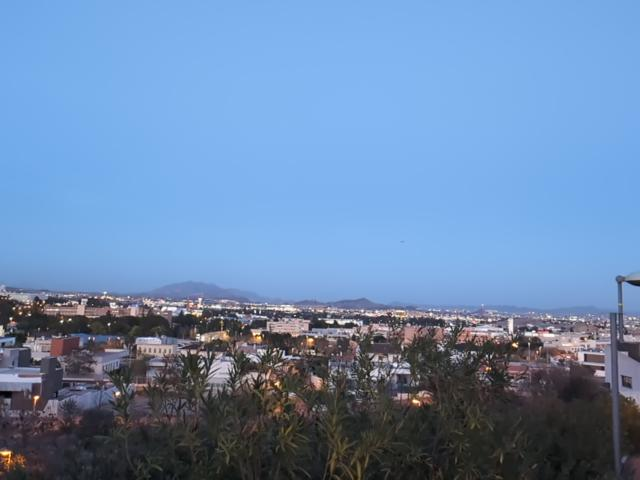
\includegraphics[width=0.7\textwidth]{images_calibracion/Paisaje.png} 
    \caption{Paisaje sobre el que triangular.}
    \label{fig:paisaje}
\end{figure}

El primer paso para hacer la triangulación es elegir tres puntos distinguidos. En mi caso y debido a lo sencillos que son de reconocer serán:
\begin{itemize}
    \item[] $NC$: El poste del centro comercial Nueva Condomina
    \item[] $TH$: El psote del centro comercial Thader
    \item[] $MA$: El Cristo de Monteagudo
\end{itemize}
Para medir su distancia angular de la forma más precisa posible primero debemos fijar una línea recta sobre la cual tomar las medidas. En mi caso tomaré la línea del horizonte \ref{fig:paisaje_angulos}
\begin{figure}[H]
    \centering
    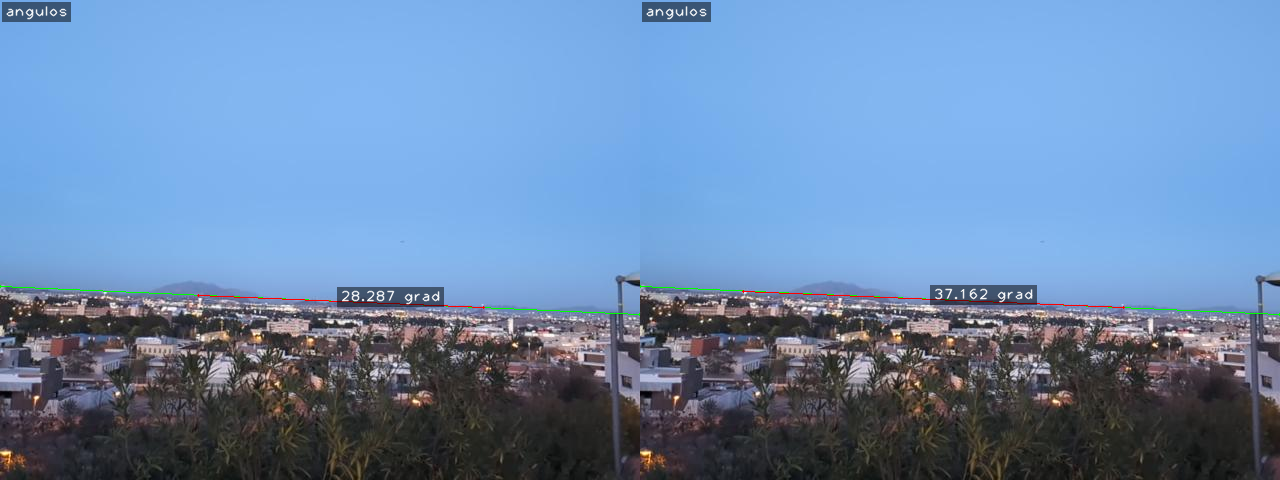
\includegraphics[width=1\textwidth]{images_calibracion/Paisaje_angulos.png} 
    \caption{Midiendo ángulos.}
    \label{fig:paisaje_angulos}
\end{figure}
Eligiendo los puntos de esta línea (verde) más cercanos a los puntos seleccionados podemos determinar que el ángulo $NC-MA$ es de $37.162^{\circ}$ y el ángulo $TH-MA$ es de $28.287^{\circ}$. Con acceso a las distancias relativas entre estos puntos y conociendo desde dónde he tomado esta fotografía podemos ver en la imagen \ref{fig:geogebra_angulos} que el error absoluto no llega a los $0.6^{\circ}$. 
\begin{figure}[H]
    \centering
    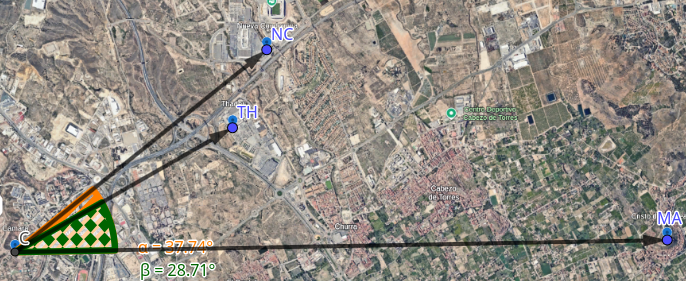
\includegraphics[width=0.8\textwidth]{images_calibracion/Angulos_Geogebra.png} 
    \caption{Ángulos reales.}
    \label{fig:geogebra_angulos}
\end{figure}

Utilizando Google Earth para calcular las distancias entre los tres puntos, los ángulos medidos y el Teorema del Ángulo exterior tenemos ya todo lo necesario para terminar la triangulación.
El último fragmento de código del notebook 'calibracion.ipynb' calcula los respectivos centros y radios de las dos circunferencias en cuya intersección se encuentra el punto desde el que se toma la fotografía, fijando el punto $TH$ como origen de coordenadas y el eje $TH \rightarrow MA$ como dirección positiva del eje de abcisas.
Trasladando los datos a la calculadora gráfica de Geogebra y teniendo en cuenta la posición relativa de los puntos observados para desambiguar entre las dos posibles intersecciones obtenemos una aproximación al punto real con una precisión de unos $89$ metros \ref{fig:geogebra_triangulacion}.
\begin{figure}[H]
    \centering
    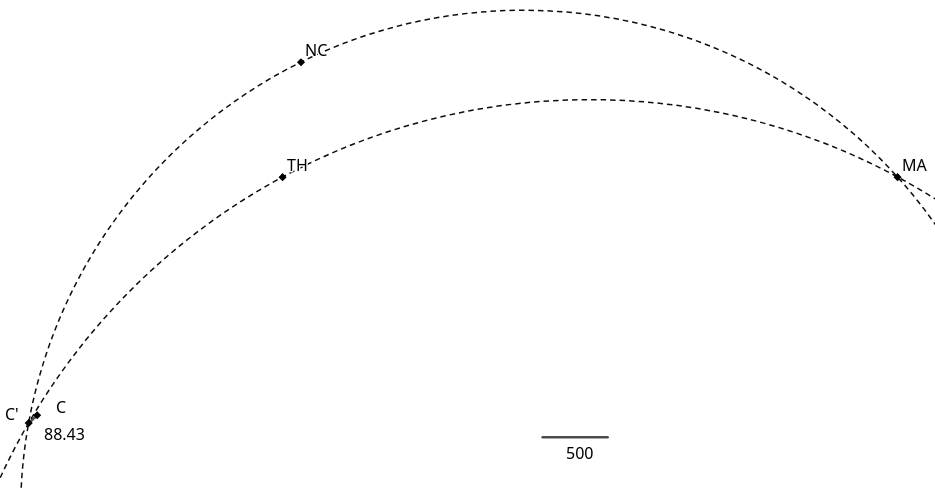
\includegraphics[width=0.8\textwidth]{images_calibracion/Triangulacion_Geogebra.png} 
    \caption{Triangulación.}
    \label{fig:geogebra_triangulacion}
\end{figure}

\newpage

% Sección 3: Filtros
\section{Filtros}

\subsection{Filtros: Marco Teórico}

Un filtro de imagen es una transformación que se aplica a la misma para modificar o extraer algunos aspectos de la misma. 
El valor del filtrado para cada píxel se calcula a partir de un entorno o vecindad del mismo.
Los filtros se pueden clasificar según de la manera que se apliquen o de los efectos que tengan en la iamgen.
Para el desarrollo de este ejercicio destacamos las clases:
\begin{itemize}
    \item[--] Filtros de suavizado: atenuan el ruido y revierten la discretización de la imagen. De ahí el calificativo de 'suave', ya que aproximan un conjunto de valores discretos a una curva suave.
    \item[--] Filtros de detección de bordes: resaltan los perfiles de los objetos de una imagen destacando las transiciones entre ellos.
    \item[--] Filtros lineales: el valor de un pixel se calcula como combinación lineal de sus elementos vecinos.
    \item[--] Filtros no lineales: el cálculo del filtro no se realiza como una combinación lineal de sus elementos vecinos.
\end{itemize}
En esta sección comentaremos el funcionamiento de los filtros y en la siguiente hablaremos de sus efectos en la imagen.

\subsubsection{Filtro de medias}

El filtro de medias es un filtro lineal de suavizado. 
Para cada píxel, se calcula como una operación de promedio sobre una vecindad del mismo.
Esta vecindad es un área $3\times 3$, $5\times 5$... centrada en el píxel.
Un ejemplo de cálculo del filtro para una vecindad $3\times 3$ en una imagen con un solo canal de color podría ser:
$$
\begin{bmatrix}
0 & 100 & 133 \\
24 & 112 & 67 \\
3 & 129 & 33
\end{bmatrix}
\Rightarrow \frac{0+100+133+24+112+67+3+129+33}{9} = 66,78
$$
Para píxeles del borde existen formas de adaptar sus vecindades como completar con ceros o sustituirlas por los rectángulos sobrantes.
La complejidad óptima en tiempo y en espacio para el cálculo de este filtro para una imagen de $n\times m$ píxeles con vecindades de tamaño $k \times k$ es $O(n\times m)$. 
Para conseguir esta complejidad es necesario mantener una matriz auxiliar de sumas acumuladas para calcular las sumas en rangos en $O(1)$.

\subsubsection{Filtro Gaussiano}
El filtro Gaussiano es otro filtro lineal de suavizado que se define mediante una función gaussiana discreta. Dadas las coordenadas relativas (x,y) de un píxel al central, el coeficiente por el que se multiplica es:
$$
    G(x,y) = \frac{1}{2 \pi \sigma^2}e^\frac{-x^2-y^2}{2\sigma^2}
$$
donde $\sigma$ es la desviación típica de la distribución y el parámetro que determina la cantidad de suavizado.

La principal diferencia de este filtro con el anterior es que mientras que en el filtro de medias todos los píxeles tienen el mismo peso, el filtro gaussiano da mayor peso a los píxeles más próximos al central.
Además, la distribución gaussiana en dos dimensiones tiene dos propiedades muy deseables:
\begin{enumerate}
    \item Separabilidad: el filtro puede ser descompuesto en dos filtros unidimensionales $G(x,y) = G_1(x) \times G_2(y)$ donde $G_1$ y $G_2$ son las distribuciones para las filas y las columnas respectivamente.
    \item Cascading: dadas dos distribuciones gaussianas con desviaciones típicas $\sigma_1$ y $\sigma_2$ se cumple que la distibución gaussiana con desviación típica 
\end{enumerate}


\newpage

% Sección 4: Clasificador
\section{Clasificador}
Aquí se hablará sobre los clasificadores utilizados para la tarea específica. Se puede incluir la descripción de los algoritmos empleados, su rendimiento y los datos con los que se entrenaron.


% Incluir la imagen
\begin{figure}[h!]
    \centering
    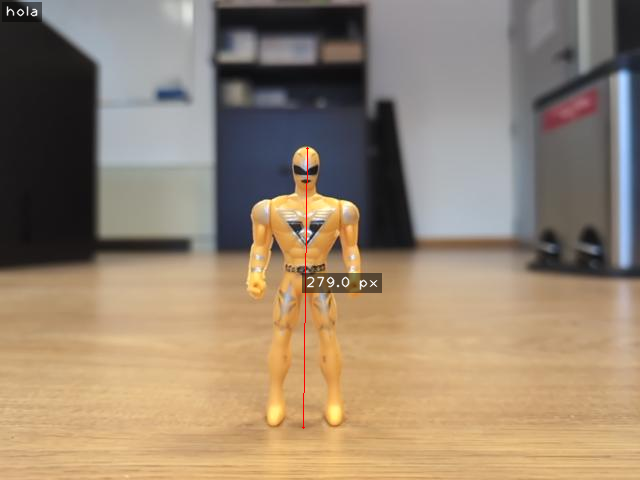
\includegraphics[width=0.7\textwidth]{images_calibracion/Altura_objeto.png} 
    \caption{Una imagen de ejemplo.}
    \label{fig:imagen_ejemplo}
\end{figure}

Como se puede ver en la \ref{fig:imagen_ejemplo}, esta es una imagen de ejemplo que se utiliza en el documento.

\end{document}